
In this section a background of the theory behind the combinatorial games studied for this thesis is provided. In addition to this, the notation introduced here is used throughout the thesis. 

\subsection{Partially Ordered Sets}
This thesis is about a type of combinatorial games called \emph{poset games}. In order to be able to introduce the theory of these games, we must first define what a poset is.
\begin{defn}[Partially Ordered Sets{\cite[p.~278]{stanley2011}}]
A \emph{partially ordered set} (\emph{poset}) $(P,\le)$ is a set with a binary order relation $\le$ satisfying the following three axioms:
\begin{enumerate}
\item For all $t\in P$, $t\le t$ (reflexivity).
\item If $s\le t$ and $t\le s$,then $s=t$ (antisymmetry).
\item If $s\le t$ and $t\le u$,then $s\le u$ (transitivity).
\end{enumerate}
\end{defn}
~\\
We use the obvious notation $t\ge s$ to mean $s\le t$, $s<t$ to mean $s\le t$ and $s\ne t$, and $t>s$ to mean $s<t$. We say that two elements $s$ and $t$ of $P$ are \emph{comparable} if $s\le t$ or $t\le s$, otherwise $s$ and $t$ are \emph{incomparable}.
\\
We define an \emph{interval} $[p,q]$ of a poset to be $\{x\in P\;|\;p\le x\le q\}$. We say that $v$ covers $u$ if $[u,v]=\{u,v\}$, and we denote this by $u\lessdot v$.
\\\\
In a partizan element removal game, every element must have a color.
%\\
\begin{defn}[Colored Posets]
A \emph{colored poset} is a poset where each element has a color of either black or white.
\end{defn}
\begin{ex}{}
\label{ex:posets}
An example of a regular and a colored poset. %The elements higher up are greater than those lower down. The greatest element is comparable to all other elements, but the elements second highest up are not comparable to each other.
\\
\begin{minipage}[b]{0.495\textwidth}
%\begin{figure}[h]
\centering
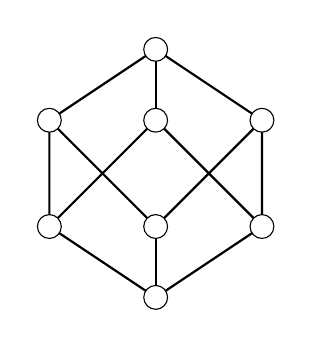
\begin{tikzpicture}[scale=.45]
  \draw[thick] (0,0) -- (-3,2) -- (-3,5) -- (0,7) -- (3,5) -- (3,2) -- (0,0);
  \draw[thick] (3,5) -- (0,2) -- (-3,5);
  \draw[thick] (0,0) -- (0,2);
  \draw[thick] (-3,2) -- (0,5) -- (3,2);
  \draw[thick] (0,5) -- (0,7);
  \node (zero) at (0,0) {\tikz\draw[black,fill=white] (0,0) circle (1ex);};
  \node (1) at (-3,2) {\tikz\draw[black,fill=white] (0,0) circle (1ex);};
  \node (2) at (0,2) {\tikz\draw[black,fill=white] (0,0) circle (1ex);};
  \node (3) at (3,2) {\tikz\draw[black,fill=white] (0,0) circle (1ex);};
  \node (4) at (-3,5) {\tikz\draw[black,fill=white] (0,0) circle (1ex);};
  \node (5) at (0,5) {\tikz\draw[black,fill=white] (0,0) circle (1ex);};
  \node (6) at (3,5) {\tikz\draw[black,fill=white] (0,0) circle (1ex);};
  \node (7) at (0,7) {\tikz\draw[black,fill=white] (0,0) circle (1ex);};
\end{tikzpicture}
\captionof{figure}{Example of a poset.}
%\end{figure}
\end{minipage}
\begin{minipage}{0.01\textwidth}
~
\end{minipage}
\begin{minipage}[b]{0.495\textwidth}
%\begin{figure}[H]
\centering
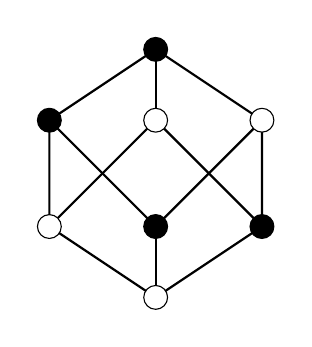
\begin{tikzpicture}[scale=.45]
  \draw[thick] (0,0) -- (-3,2) -- (-3,5) -- (0,7) -- (3,5) -- (3,2) -- (0,0);
  \draw[thick] (3,5) -- (0,2) -- (-3,5);
  \draw[thick] (0,0) -- (0,2);
  \draw[thick] (-3,2) -- (0,5) -- (3,2);
  \draw[thick] (0,5) -- (0,7);
  \node (zero) at (0,0) {\tikz\draw[black,fill=white] (0,0) circle (1ex);};
  \node (1) at (-3,2) {\tikz\draw[black,fill=white] (0,0) circle (1ex);};
  \node (2) at (0,2) {\tikz\draw[black,fill=black] (0,0) circle (1ex);};
  \node (3) at (3,2) {\tikz\draw[black,fill=black] (0,0) circle (1ex);};
  \node (4) at (-3,5) {\tikz\draw[black,fill=black] (0,0) circle (1ex);};
  \node (5) at (0,5) {\tikz\draw[black,fill=white] (0,0) circle (1ex);};
  \node (6) at (3,5) {\tikz\draw[black,fill=white] (0,0) circle (1ex);};
  \node (7) at (0,7) {\tikz\draw[black,fill=black] (0,0) circle (1ex);};
\end{tikzpicture}
\captionof{figure}{Example of a colored poset.}
%\end{figure}
\end{minipage}
\end{ex}
~\\%\newpage
In particular, this thesis focuses on poset games with a specific coloring called chess-coloring.
\\
\begin{minipage}[t]{0.40\textwidth}
\begin{defn}[Chess-Colored Posets]
A \emph{chess-colored poset} is a colored poset such that no element covers an element of the same color. Equivalently we may regard $P=W\cup B$ as a bipartite graph, with white vertices $W$ and black vertices $B$, with the cover relation as an edge relation.
\\
To avoid confusion, we will assume that the least element is colored white when there is only one smallest element.
\end{defn}
\end{minipage}
\begin{minipage}{0.04\textwidth}
~
\end{minipage}
%\begin{figure}[h]
\begin{minipage}[t]{0.55\textwidth}
\begin{ex}{}~
\\
\begin{center}
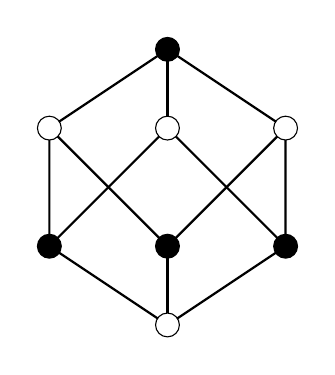
\begin{tikzpicture}[baseline=0.65ex,scale=.5]
  \draw[thick] (0,0) -- (-3,2) -- (-3,5) -- (0,7) -- (3,5) -- (3,2) -- (0,0);
  \draw[thick] (3,5) -- (0,2) -- (-3,5);
  \draw[thick] (0,0) -- (0,2);
  \draw[thick] (-3,2) -- (0,5) -- (3,2);
  \draw[thick] (0,5) -- (0,7);
  \node (zero) at (0,0) {\tikz\draw[black,fill=white] (0,0) circle (1ex);};
  \node (1) at (-3,2) {\tikz\draw[black,fill=black] (0,0) circle (1ex);};
  \node (2) at (0,2) {\tikz\draw[black,fill=black] (0,0) circle (1ex);};
  \node (3) at (3,2) {\tikz\draw[black,fill=black] (0,0) circle (1ex);};
  \node (4) at (-3,5) {\tikz\draw[black,fill=white] (0,0) circle (1ex);};
  \node (5) at (0,5) {\tikz\draw[black,fill=white] (0,0) circle (1ex);};
  \node (6) at (3,5) {\tikz\draw[black,fill=white] (0,0) circle (1ex);};
  \node (7) at (0,7) {\tikz\draw[black,fill=black] (0,0) circle (1ex);};
\end{tikzpicture}
%\caption{Example of a chess-colored poset.}
\captionof{figure}{Example of a chess-colored poset.}
\end{center}
\end{ex}
\end{minipage}
%\end{figure}
%\begin{minipage}{0.05\textwidth}
%~
%\end{minipage}
%\begin{minipage}[b]{0.475\textwidth}
%\centering
%\begin{tikzpicture}[scale=.5]
%  \node (zero) at (0,0) {\tikz\draw[black,fill=white] (0,0) circle (.5ex);};
%  \node (1) at (-3,2) {\tikz\draw[black,fill=black] (0,0) circle (.5ex);};
%  \node (2) at (0,2) {\tikz\draw[black,fill=black] (0,0) circle (.5ex);};
%  \node (3) at (3,2) {\tikz\draw[black,fill=black] (0,0) circle (.5ex);};
%  \node (4) at (-3,5) {\tikz\draw[black,fill=white] (0,0) circle (.5ex);};
%  \node (5) at (0,5) {\tikz\draw[black,fill=white] (0,0) circle (.5ex);};
%  \node (6) at (3,5) {\tikz\draw[black,fill=white] (0,0) circle (.5ex);};
%  \node (7) at (0,7) {\tikz\draw[black,fill=black] (0,0) circle (.5ex);};
%  \draw[thick] (zero) -- (1) -- (4);
%  \draw[thick] (6) -- (2) -- (zero);
%  \draw[thick] (5) -- (7);
%  \draw[thick] (1) -- (5) -- (7);
%  \draw[thick] (zero) -- (3);
%\end{tikzpicture}
%\captionof{figure}{Example of a (chess-colored) tree poset.}
%\end{minipage}
%%\end{figure}
%\\\\
%%\begin{minipage}[b]{0.5\textwidth}
%\begin{defn}[Tree Posets]
%A \emph{tree poset} is a poset that, when regarded as a graph with the cover relations as undirected edges, has no cycles. A forest poset is a poset where all components of the poset (when the poset is regarded as a graph with the cover relations as undirected edges) are tree posets.
%\end{defn}
%%\end{minipage}
%%\begin{minipage}{0.1\textwidth}
%%~
%%\end{minipage}
%%\begin{figure}[h]
%%
\subsubsection{Young Diagrams}
This thesis mainly focuses on an object called \emph{Young diagram}. We will formally define exactly what a Young diagram is in Definition \ref{def:lambda}, but before that we need the following definition:
\begin{defn}
\label{def:lambda}
Let $\lambda=(\lambda_1,\dots,\lambda_k)$ be a weakly decreasing sequence of positive integers, i.e., $\lambda_1\ge \lambda_2\ge\dots\ge \lambda_k$. We say that $\lambda$ partitions $n$, denoted by $\lambda\vdash n$, if $\sum_{i=1}^k\lambda_i =n$.
\end{defn}
%~
\begin{defn}[Young Diagrams%{\cite[p.~155]{hk2002}}
]
A \emph{Young diagram} is a collection of boxes arranged in left-justified rows with a weakly decreasing number of boxes in each row. If the number of boxes is $n$ and $\lambda\vdash n$, we say that $\lambda$ generate a Young diagram with $\lambda_1$ boxes in the first row, $\lambda_2$ boxes in the second row,$\dots$, $\lambda_k$ in the $k$'th row.
Moreover, a Young diagram can always be represented as a poset.
\end{defn}
~\\
This definition is best illustrated with an example. 
\begin{ex}{}
With $\lambda=(7,5,2,2,1)$ we have the Young diagram in Figure \ref{fig:youngex} and the corresponding representation as a poset in Figure \ref{fig:youngposetex}.
\\
%\begin{picex}{}
\begin{minipage}[b]{0.45\textwidth}
%\begin{math}
\centering
\begin{tabular}{ | c | c | c | c | c | c | c |}
\hline
~&~&~&~&~&~&~\\
\hline
~&~&~&~&~\\
\cline{1-5}
~&~\\
\cline{1-2}
~&~\\
\cline{1-2}
~\\
\cline{1-1}
\end{tabular}
%\end{math}
\captionof{figure}{Young diagram generated by $\lambda=(7,5,2,2,1)$.}
\label{fig:youngex}
\end{minipage}
%\begin{center}
%\begin{figure}
%\begin{Young}
 %& & & & & & \cr
 %& & & & \cr
 %& \cr
 %& \cr
 %\cr
%\end{Young}
%\end{figure}
%\end{center}
\begin{minipage}{0.05\textwidth}
~%This Young diagram can also be represented as the following poset:
\end{minipage}
\begin{minipage}[b]{0.50\textwidth}
\centering
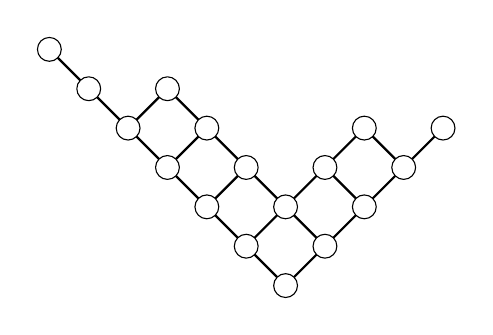
\begin{tikzpicture}[scale=.5]
  \draw[thick] (0,0) -- (-1,1) -- (-2,2) -- (-3,3) -- (-4,4) -- (-5,5) -- (-6,6);
  \draw[thick] (1,1) -- (0,2) -- (-1,3) -- (-2,4) -- (-3,5);
  \draw[thick] (2,2) -- (1,3);
  \draw[thick] (3,3) -- (2,4);
  \draw[thick] (0,0) -- (1,1) -- (2,2) -- (3,3) -- (4,4);
  \draw[thick] (-1,1) -- (0,2) -- (1,3) -- (2,4);
  \draw[thick] (-2,2) -- (-1,3);
  \draw[thick] (-3,3) -- (-2,4);
  \draw[thick] (-4,4) -- (-3,5);
  \node (zero) at (0,0) {\tikz\draw[black,fill=white] (0,0) circle (1ex);};
  \node (1) at (-1,1) {\tikz\draw[black,fill=white] (0,0) circle (1ex);};
  \node (2) at (-2,2) {\tikz\draw[black,fill=white] (0,0) circle (1ex);};
  \node (3) at (-3,3) {\tikz\draw[black,fill=white] (0,0) circle (1ex);};
  \node (4) at (-4,4) {\tikz\draw[black,fill=white] (0,0) circle (1ex);};
  \node (5) at (-5,5) {\tikz\draw[black,fill=white] (0,0) circle (1ex);};
  \node (6) at (-6,6) {\tikz\draw[black,fill=white] (0,0) circle (1ex);};
  \node (7) at (1,1) {\tikz\draw[black,fill=white] (0,0) circle (1ex);};
  \node (8) at (0,2) {\tikz\draw[black,fill=white] (0,0) circle (1ex);};
  \node (9) at (-1,3) {\tikz\draw[black,fill=white] (0,0) circle (1ex);};
  \node (10) at (-2,4) {\tikz\draw[black,fill=white] (0,0) circle (1ex);};
  \node (11) at (-3,5) {\tikz\draw[black,fill=white] (0,0) circle (1ex);};
  \node (12) at (2,2) {\tikz\draw[black,fill=white] (0,0) circle (1ex);};
  \node (13) at (1,3) {\tikz\draw[black,fill=white] (0,0) circle (1ex);};
  \node (14) at (3,3) {\tikz\draw[black,fill=white] (0,0) circle (1ex);};
  \node (15) at (2,4) {\tikz\draw[black,fill=white] (0,0) circle (1ex);};
  \node (16) at (4,4) {\tikz\draw[black,fill=white] (0,0) circle (1ex);};
\end{tikzpicture}
\captionof{figure}{Poset of the Young diagram generated by $\lambda=(7,5,2,2,1)$.}
\label{fig:youngposetex}
\end{minipage}
\end{ex}
In analogy with the previous definitions, a colored Young diagram is a Young diagram where each box has a color of either black or white, and a chess-colored Young diagram is a Young diagram where no adjacent boxes have the same color.
%\\
\begin{ex}{}
With $\lambda=(7,5,2,2,1)$ as before, we have the chess-colored Young diagram and the corresponding chess-colored poset in Figures \ref{fig:chessyoung} and \ref{fig:chessyoungposet} respectively.
\\
%\begin{picex}{}
\begin{minipage}[b]{0.45\textwidth}
%\begin{figure}[H]
\centering
\begin{tabular}{ | c | c | c | c | c | c | c |}
\hline
~&\cellcolor[gray]{0}&~&\cellcolor[gray]{0}&~&\cellcolor[gray]{0}&~\\
\hline
\cellcolor[gray]{0}&~&\cellcolor[gray]{0}&~&\cellcolor[gray]{0}\\
\cline{1-5}
~&\cellcolor[gray]{0}\\
\cline{1-2}
\cellcolor[gray]{0}&~\\
\cline{1-2}
~\\
\cline{1-1}
\end{tabular}
\captionof{figure}{Chess-colored Young diagram generated by $\lambda=(7,5,2,2,1)$.}
\label{fig:chessyoung}
%\end{figure}
\end{minipage}
\begin{minipage}{0.05\textwidth}
~
\end{minipage}
\begin{minipage}[b]{0.5\textwidth}
%\begin{figure}[H]
\centering
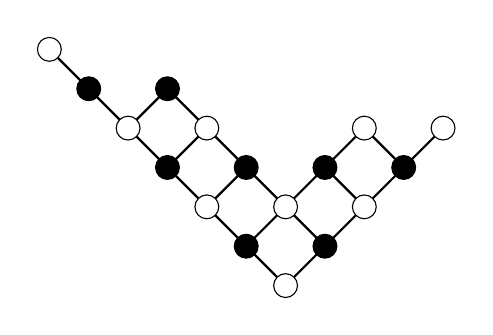
\begin{tikzpicture}[scale=.5]
  \draw[thick] (0,0) -- (-1,1) -- (-2,2) -- (-3,3) -- (-4,4) -- (-5,5) -- (-6,6);
  \draw[thick] (1,1) -- (0,2) -- (-1,3) -- (-2,4) -- (-3,5);
  \draw[thick] (2,2) -- (1,3);
  \draw[thick] (3,3) -- (2,4);
  \draw[thick] (0,0) -- (1,1) -- (2,2) -- (3,3) -- (4,4);
  \draw[thick] (-1,1) -- (0,2) -- (1,3) -- (2,4);
  \draw[thick] (-2,2) -- (-1,3);
  \draw[thick] (-3,3) -- (-2,4);
  \draw[thick] (-4,4) -- (-3,5);
  \node (zero) at (0,0) {\tikz\draw[black,fill=white] (0,0) circle (1ex);};
  \node (1) at (-1,1) {\tikz\draw[black,fill=black] (0,0) circle (1ex);};
  \node (2) at (-2,2) {\tikz\draw[black,fill=white] (0,0) circle (1ex);};
  \node (3) at (-3,3) {\tikz\draw[black,fill=black] (0,0) circle (1ex);};
  \node (4) at (-4,4) {\tikz\draw[black,fill=white] (0,0) circle (1ex);};
  \node (5) at (-5,5) {\tikz\draw[black,fill=black] (0,0) circle (1ex);};
  \node (6) at (-6,6) {\tikz\draw[black,fill=white] (0,0) circle (1ex);};
  \node (7) at (1,1) {\tikz\draw[black,fill=black] (0,0) circle (1ex);};
  \node (8) at (0,2) {\tikz\draw[black,fill=white] (0,0) circle (1ex);};
  \node (9) at (-1,3) {\tikz\draw[black,fill=black] (0,0) circle (1ex);};
  \node (10) at (-2,4) {\tikz\draw[black,fill=white] (0,0) circle (1ex);};
  \node (11) at (-3,5) {\tikz\draw[black,fill=black] (0,0) circle (1ex);};
  \node (12) at (2,2) {\tikz\draw[black,fill=white] (0,0) circle (1ex);};
  \node (13) at (1,3) {\tikz\draw[black,fill=black] (0,0) circle (1ex);};
  \node (14) at (3,3) {\tikz\draw[black,fill=black] (0,0) circle (1ex);};
  \node (15) at (2,4) {\tikz\draw[black,fill=white] (0,0) circle (1ex);};
  \node (16) at (4,4) {\tikz\draw[black,fill=white] (0,0) circle (1ex);};
\end{tikzpicture}
\captionof{figure}{Chess-colored poset of the Young diagram in figure \ref{fig:chessyoung}.}
\label{fig:chessyoungposet}
%\end{figure}
\end{minipage}
\end{ex}


\subsection{Combinatorial Game Theory}
This thesis deals with combinatorial game theory, an area which studies sequential games with perfect information, that is, games where the players play in turns and where they have complete knowledge of the game, i.e., know all possible game options for all players. 
\\
In particular, the thesis will focus on two-player partizan combinatorial games, in which the game options of the two players can be different. Furthermore, we call the two players Left and Right (or White and Black or Blue and Red).
\\
In general, a combinatorial game has \emph{positions}, and at any given position every player has a set of \emph{options} of moving to a new position. Under normal play convention a player loses if they have no options available at their turn to move.
%\\
\begin{defn}[Partizan Game Position{\cite[p.~71]{onag}}]
A position in a partizan game is defined by its left and right options, and we denote it by $G=\{L|R\}$, where $L$ and $R$ are the sets of left and right options respectively. 
\end{defn}
~\\
Since we will be using the notation used by Conway\cite{onag}, the notation above will not always be used, and we will instead often abuse it by writing $G=\{G_1,G_2,G_3|H_1,H_2\}$ as short for $G=\left\{\{G_1,G_2,G_3\}|\{H_1,H_2\}\right\}$, and in the general case $G=\{G^L|G^R\}$.
\\
Following this we will introduce some notation for the games depending on the winner and who starts.
%\\
\begin{defn}[Value Notation{\cite[p.~73]{onag}}]
\label{def:value}
~
\begin{itemize}
\item $G>0$ ($G$ is \emph{positive}) if there is a winning strategy for Left.
\item $G<0$ ($G$ is \emph{negative}) if there is a winning strategy for Right.
\item $G=0$ ($G$ is \emph{zero}) if there is a winning strategy for the second player to move.
\item $G\parallel0$ ($G$ is \emph{fuzzy} to zero) if there is a winning strategy for first player move.
\end{itemize}
\end{defn}
~\\
This notation is easy to understand with help of some examples.
%\\
\begin{ex}{}
Consider the simplest possible game, the game with no options for either player, i.e., $G_1=\{|\}$. We obviously have $G_1=0$, since the first player has no options to play and therefore loses. This game is denoted by $0:=\{|\}$.
\\
Now consider the game where Left has the option to move to $0$, but Right still has no options, i.e., $G_2=\{0|\}$. Here we have that $G_2>0$ since either Left starts and moves to $0$, and then Right has no option and loses, or Right starts and has no options and therefore loses, i.e., Left has a winning strategy. This game is denoted by $1:=\{0|\}$. Similarly we have that the game $-1<0$ where $-1$ is defined as $-1:=\{|0\}$.
\\
Finally, consider the game where both players have the option to move to $0$, i.e., $G_3=\{0|0\}$. We now have $G_3\parallel0$ since both players have the option to move to $0$, where the second player then will lose. This game is denoted as $*:=\{0|0\}$.
\end{ex}
%\newpage
~\\
The value notation of Definition \ref{def:value} can be combined and extended in the following way.
\begin{defn}[Extended Value Notation{\cite[p.~73]{onag}}]
\label{def:extvalue}~
\begin{itemize}
\item If $G\ge0$, then Left always wins if Left is the second player to move.
\item If $G\le0$, then Right always wins if Right is the player second to move.
\item If $G\rhd0$, then Left always wins if Left is the first player to move.
\item If $G\lhd0$, then Right always wins if Right is the first player to move.
\end{itemize}
\end{defn}
~\\
In addition to the value notations, it is also possible to add and subtract games.
\begin{defn}[Addition and Negation{\cite[p.~73]{onag}}]
\begin{align*}
G+H&=\left\{G^L+H,G+H^L\middle|G^R+H,G+H^R\right\}\\
-G&=\left\{-G^R\middle|-G^L\right\}
\end{align*}
\end{defn}
~\\
Informally, we can note that addition of two games is the same as playing in both games at the same time, and the negation of a game is the game with reversed roles of Left and Right. Combining these, it is possible to subtract games as $G-H=G+(-H)$. 
\\
Using this, we define the following relations between games:
\begin{defn}[Game Relations{\cite[p.~78]{onag}}]
~
\begin{itemize}
\item $G>H$ iff $G-H>0$.
\item $G<H$ iff $G-H<0$.
\item $G=H$ iff $G-H=0$.
\item $G\parallel H$ iff $G-H\parallel0$.
\end{itemize}
\end{defn}
~\\
Using these relations, which can be combined and extended as the extended notation of Definition \ref{def:extvalue}, we can define what a \emph{dominated} option is.
\begin{defn}[Dominated Options{\cite[p.~110]{onag}}]
\label{def:dominate}
For a game we say that a left option $G^{L_1}$ is dominated by another left option option $G^{L_0}$ if $G^{L_1}\le G^{L_0}$. Similarly, a right option $G^{R_1}$ is dominated by another right option $G^{R_0}$ if $G^{R_1}\ge G^{R_0}$.
\end{defn}
~\\
In fact, an important property of a game is that you always can remove any dominated options{\cite[p.~110]{onag}}.
\begin{thm}
\label{thm:domopt}
Let $G=\left\{G^{L_0},G^{L_1},\dots|G^{R_0},G^{R_1}\dots,\right\}$. 
\begin{itemize}
\item If $G^{L_0}\le G^{L_1}$, then $G=G'$, where $G'=\left\{G^{L_1},\dots|G^{R_0},G^{R_1}\dots,\right\}$.
\item If $G^{R_0}\ge G^{R_1}$, then $G=G''$, where $G''=\left\{G^{L_0},G^{L_1},\dots|G^{R_1}\dots,\right\}$.
\end{itemize}
\end{thm}
~\\
A significant class of games are the \emph{short} games.
\begin{defn}[Short Games{\cite[p.~3]{lip}\cite[p.97]{onag}}]
A game G is short if only a finite number of positions can be reached and a position may never be repeated.
\end{defn}
~\\
Moreover, every short game $G$ has a unique simplest form. This is called $G$'s canonical form{\cite[p.~78]{lip}}. It is possible to reduce any short game to its canonical form by just removing dominated and \emph{reversible} options{\cite[p.~111]{onag}}.
\\\\
A methodology that is extremely useful when proving properties of games is \emph{Conway induction}.
\begin{thm}[Conway Induction{\cite[p.~5]{onag}}]
\label{thm:conind}
Let $P$ be a property which games might have, such that any game $G$ has property $P$ whenever all left and right options of $G$ have this property. Then every game has property $P$.
\end{thm}
~\\
The methodology using Conway induction makes it possible to prove that a game has a property by assuming that all its options have this property, and from this proving that the game itself has it. This methodology is using that the definitions of games are inductive.
\subsubsection{Numbers}
\label{section:numbers}
Another important property and concept in combinatorial games is that of numbers, which is a class of games with some special characteristics. 
%\\
\begin{defn}[Numbers{\cite[p.~91]{lip}}]
A number is any game $x$ such that all $x^L<x<x^R$ and $x^L$ and $x^R$ are numbers.
For short games, we can, equivalently, for $j>0$ and $m$ odd, define a number as
\begin{equation}
\frac{m}{2^j}=\left\{\frac{m-1}{2^j}\Bigg|\frac{m+1}{2^j}\right\}.
\label{eq:number}
\end{equation}
\label{def:number}
\end{defn}
~\\
It should also be noted that all games are not numbers. For $*=\{0|0\}$ we have $G^L=0=G^R$, and hence $G^L\not<G^R$, i.e., $*$ is not a number.
\\
Equation (\ref{eq:number}) can be generalized to recognize when $G$ is a number even if it is not in canonical form. For this, we need to define what the \emph{simplest number} is.
%\\
\begin{defn}[Simplest Number{\cite[p.~93]{lip}}]
\label{def:simpnum}
For $x^L<x^R$, the simplest number $x$ between $x^L$ and $x^R$ is given by the following:
\begin{itemize}
\item If there are integer(s) $n$ such that $x^L<n<x^R$, $x$ is the one that is smallest in absolute value.
\item Otherwise, $x$ is the number of the form $\frac{i}{2^j}$ between $x^L$ and $x^R$ for which $j$ is minimal.
\end{itemize}
\end{defn}
%~
\begin{thm}[Numbers{\cite[p.~93]{lip}}]
\label{thm:number}
If all options of a game $G$ are numbers and all $G^L<G^R$, then $G$ is the simplest number $x$ satisfying $G^L<x<G^R$. 
\end{thm}
~\\
This, together with Definition \ref{def:dominate} and Theorem \ref{thm:domopt}, yields that a game that is equal to a number is equal to the game consisting of only its greatest left options and smallest right options, i.e., 
$G\equiv\left\{G^{L_0},G^{L_1},\dots|G^{R_0},G^{R_1}\dots,\right\}=\left\{G^{L_0}|G^{R_0}\right\}\equiv G'$ if $G^{L_0}\ge G^{L_i}$ and $G^{R_0}\le G^{R_j}$ for $i,j>0$. 
\\
It should also be noted that equation (\ref{eq:number}) is a number for integers $j>0$ and $m$, regardless if $m$ is odd or not.

\subsubsection{Hackenbush}
A game with properties similar to the ones studied in this thesis is \emph{Blue-Red Hackenbush}. Hackenbush is a partizan two-player game that may be played on any configuration of colored line segments connected to one another by their endpoints and to a "ground" line. In the Blue-Red Hackenbush, the line segments are colored either blue or red. It is played by, in turns, removing a line segment of your color, by which all segments that are unconnected to the ground vanishes, until a player has no move left.
\begin{ex}{}
\label{ex:hack}
An example of a game of Blue-Red Hackenbush and gameplay on that game.
\begin{figure}[H]
\centering
{\Large
$
\begin{tikzpicture}[baseline=-0.65ex,scale=0.5]
    \draw[densely dashed] (-1,-1) -- (1,-1);
    \node[hackennode] (middle) at ( 0,   0) {};
    \node[hackennode] (left)   at (-0.5,-1) {};
    \node[hackennode] (right)  at ( 0.5,-1) {};
    \node[hackennode] (top)    at ( 0,   1) {};
    \node[hackennode] (top2)   at ( 0,   2) {};

    \draw[hackenline,blue]
        (left) -- (middle) -- (right);
    \draw[hackenline,red!75]
        (middle) -- (top);
    \draw[hackenline,red!75]
        (top) -- (top2);
\end{tikzpicture}
=
\left\{
\begin{tikzpicture}[baseline=-0.65ex,scale=0.5]
    \draw[densely dashed] (-0.5,-1) -- (1,-1);
    \node[hackennode] (middle) at ( 0,   0) {};
    \node[hackennode] (right)  at ( 0.5,-1) {};
    \node[hackennode] (top)    at ( 0,   1) {};
    \node[hackennode] (top2)   at ( 0,   2) {};

    \draw[hackenline,blue]
        (middle) -- (right);
    \draw[hackenline,red!75]
        (middle) -- (top);
    \draw[hackenline,red!75]
        (top) -- (top2);
\end{tikzpicture}
\tikz[baseline=-0.65ex,scale=0.5] \node[inner sep=0] at (0,-1) {,\,};
\begin{tikzpicture}[baseline=-0.65ex,scale=0.5]
    \draw[densely dashed] (-1,-1) -- (0.5,-1);
    \node[hackennode] (middle) at ( 0,   0) {};
    \node[hackennode] (left)   at (-0.5,-1) {};
    \node[hackennode] (top)    at ( 0,   1) {};
    \node[hackennode] (top2)   at ( 0,   2) {};

    \draw[hackenline,blue]
        (middle) -- (left);
    \draw[hackenline,red!75]
        (middle) -- (top);
    \draw[hackenline,red!75]
        (top) -- (top2);
\end{tikzpicture}
\middle|
\begin{tikzpicture}[baseline=-0.65ex,scale=0.5]
    \draw[densely dashed] (-0.5,-1) -- (1,-1);
    \node[hackennode] (middle) at ( 0,   0) {};
    \node[hackennode] (left)   at (-0.5,-1) {};
    \node[hackennode] (right)  at ( 0.5,-1) {};
    \node[hackennode] (top)    at ( 0,   1) {};

    \draw[hackenline,blue]
        (left) -- (middle) -- (right);
    \draw[hackenline,red!75]
        (middle) -- (top);
\end{tikzpicture}
\tikz[baseline=-0.65ex,scale=0.5] \node[inner sep=0] at (0,-1) {,\,};
\begin{tikzpicture}[baseline=-0.65ex,scale=0.5]
    \draw[densely dashed] (-1,-1) -- (0.5,-1);
    \node[hackennode] (middle) at ( 0,   0) {};
    \node[hackennode] (left)   at (-0.5,-1) {};
    \node[hackennode] (right)  at ( 0.5,-1) {};

    \draw[hackenline,blue]
        (left) -- (middle) -- (right);
\end{tikzpicture}
\right\}
$
}% End group with \Large
\caption{A simple game of Blue-Red Hackenbush.}
\label{fig:hackenbush}
\end{figure}
\begin{figure}[H]
{\Large
\[
\begin{tikzpicture}[baseline=-0.65ex,scale=0.5]
    \draw[densely dashed] (-1,-1) -- (1,-1);
    \node[hackennode] (middle) at ( 0,   0) {};
    \node[hackennode] (left)   at (-0.5,-1) {};
    \node[hackennode] (right)  at ( 0.5,-1) {};
    \node[hackennode] (top)    at ( 0,   1) {};
    \node[hackennode] (top2)   at ( 0,   2) {};

    \draw[hackenline,blue]
        (left) -- (middle) -- node[strike out,draw=black,line width=1,-]{}(right);
    \draw[hackenline,red!75]
        (middle) -- (top);
    \draw[hackenline,red!75]
        (top) -- (top2);
\end{tikzpicture}
\overset{L}{\longrightarrow}
\begin{tikzpicture}[baseline=-0.65ex,scale=0.5]
    \draw[densely dashed] (-1,-1) -- (0.5,-1);
    \node[hackennode] (middle) at ( 0,   0) {};
    \node[hackennode] (left)   at (-0.5,-1) {};
    \node[hackennode] (top)    at ( 0,   1) {};
    \node[hackennode] (top2)   at ( 0,   2) {};

    \draw[hackenline,blue]
        (middle) -- (left);
    \draw[hackenline,red!75]
        (middle) -- (top);
    \draw[hackenline,red!75]
        (top) -- node[strike out,draw=black,line width=1,-]{}(top2);
\end{tikzpicture}
\overset{R}{\longrightarrow}
\begin{tikzpicture}[baseline=-0.65ex,scale=0.5]
    \draw[densely dashed] (-0.5,-1) -- (1,-1);
    \node[hackennode] (middle) at ( 0,   0) {};
    \node[hackennode] (left)   at (-0.5,-1) {};
    \node[hackennode] (top)    at ( 0,   1) {};

    \draw[hackenline,blue]
        (middle) -- node [sloped,strike out,draw=black,line width=1,-]{}(left);
    \draw[hackenline,red!75]
        (middle) -- (top);
\end{tikzpicture}
\overset{L}{\longrightarrow}
\begin{tikzpicture}[baseline=-0.65ex,scale=0.5]
    \draw[densely dashed] (-1,-1) -- (0.5,-1);
\end{tikzpicture}
\]
}% End group with \Large
\caption{Example of gameplay on the Blue-Red Hackenbush in Figure \ref{fig:hackenbush} where Left player wins.}
\end{figure}
\end{ex}
It is known that every game of Blue-Red Hackenbush is a surreal number, and in particular, any \emph{finite} game of Blue-Red Hackenbush is a dyadic rational number, i.e., on the form $\frac{m}{2^j}$ where $m$ and $j>0$ are integers.
\subsubsection{Chomp}
\label{section:chomp}
\begin{minipage}[b]{0.5\textwidth}
Another game closely related to that of this thesis is the game of \emph{Chomp}. Chomp is a impartial two-player game with the usual starting position consisting of a rectangle (possibly infinite) with one poison square in the lower-left corner. A move in Chomp is to choose a square and remove this and all other squares above or to the right of it, and a player loses if they has to choose the poison square.
\end{minipage}
\begin{minipage}{0.05\textwidth}
~
\end{minipage}
\begin{minipage}[b]{0.45\textwidth}
%\begin{figure}[H]
\centering
\begin{tabular}{ | c | c | c | c | c |}
\hline
~&~&~&~&~\\
\hline
~&~&~&~&~\\
\hline
~&~&~&~&~\\
\hline
~&~&~&~&~\\
\hline
~&~&~&~&~\\
\hline
~&~&~&~&~\\
\hline
\cellcolor{red}&~&~&~&~\\
\hline
\end{tabular}
\captionof{figure}{Example of a starting position of a game of Chomp.}
\label{fig:chompstart}
%\end{figure}
\end{minipage}
\begin{ex}{}
\label{ex:chompgame}
An example of gameplay on a game of Chomp with starting position as in Figure \ref{fig:chompstart}.
\begin{figure}[H]
\centering
$
\begin{tabular}{ | c | c | c | c | c |}
\hhline{-----}
~&~&~&\cellcolor[gray]{0.8}&\cellcolor[gray]{0.8}\\
\hhline{-----}
~&~&~&\cellcolor[gray]{0.8}&\cellcolor[gray]{0.8}\\
\hhline{-----}
~&~&~&\cellcolor[gray]{0.8}&\cellcolor[gray]{0.8}\\
\hhline{-----}
~&~&~&\cellcolor[gray]{0.8}&\cellcolor[gray]{0.8}\\
\hhline{-----}
~&~&~&\cellcolor[gray]{0.8}&\cellcolor[gray]{0.8}\\
\hhline{-----}
~&~&~&\cellcolor[gray]{0.6}&\cellcolor[gray]{0.8}\\
\hhline{-----}
\cellcolor{red}&~&~&~&~\\
\hhline{-----}
\end{tabular}
\overset{L}{\longrightarrow}
\begin{tabular}{ | c | c | c | c | c |}
\hhline{---~~}
\cellcolor[gray]{0.8}&\cellcolor[gray]{0.8}&\cellcolor[gray]{0.8}\\
\hhline{---~~}
\cellcolor[gray]{0.8}&\cellcolor[gray]{0.8}&\cellcolor[gray]{0.8}\\
\hhline{---~~}
\cellcolor[gray]{0.8}&\cellcolor[gray]{0.8}&\cellcolor[gray]{0.8}\\
\hhline{---~~}
\cellcolor[gray]{0.8}&\cellcolor[gray]{0.8}&\cellcolor[gray]{0.8}\\
\hhline{---~~}
\cellcolor[gray]{0.6}&\cellcolor[gray]{0.8}&\cellcolor[gray]{0.8}\\
\hhline{---~~}
~&~&~\\
\hhline{-----}
\cellcolor{red}&~&~&~&~\\
\hhline{-----}
\end{tabular}
\overset{R}{\longrightarrow}
\begin{tabular}{ | c | c | c | c | c |}
\hhline{---~~}
~&\cellcolor[gray]{0.8}&\cellcolor[gray]{0.8}\\
\hhline{-----}
\cellcolor{red}&\cellcolor[gray]{0.6}&\cellcolor[gray]{0.8}&\cellcolor[gray]{0.8}&\cellcolor[gray]{0.8}\\
\hhline{-----}
\end{tabular}
\overset{L}{\longrightarrow}
\begin{tabular}{ | c |}
\hhline{-}
\cellcolor[gray]{0.6}\\
\hhline{-}
\cellcolor{red}\\
\hhline{-}
\end{tabular}
\overset{R}{\longrightarrow}
\begin{tabular}{ | c |}
\hline
\cellcolor{red}\\
\hline
\end{tabular}
$
\captionof{figure}{Example of gameplay in the game of Chomp with starting position as in Figure \ref{fig:chompstart} where Right player wins.}
\end{figure}
\end{ex}